%%%%%% Pfad zum Latex Header
\newcommand{\pfad}{../../../../../../xLatex/x_default/}

\input{\pfad HeadLizenzL.tex}

%%%%% Platz für eigene Imports


%%%%%


%%Variablen Thema der Stunde
\newcommand{\thema}{Herleitung der allgmeinen Tangentengleichung }
%%%%

%%%%%%%%%Header
\begin{document}
	\thispagestyle{specialchapter}
	\parindent 0pt  %% Kein Absatzeinzug
	\vspace*{-1.8cm}
	\hrule 
	\newcolumntype{L}[1]{>{\hsize=#1\hsize\raggedright\arraybackslash}X}%
	\newcolumntype{R}[1]{>{\hsize=#1\hsize\raggedleft\arraybackslash}X}%
	\newcolumntype{C}[1]{>{\hsize=#1\hsize\centering\arraybackslash}X}%
	\begin{tabularx}{\textwidth}{L{0.5} C{2.015} R{0.485}}
		\scriptsize Herr Wienands   & \large \multirow{2}{*}{\textbf{Mathematik}} &  \multirow{3}{*}{\raisebox{-\totalheight}{\includegraphics[scale=0.24]{\pfad Logo.png}}}  \\
		\scriptsize EPH & & \\
		\scriptsize \mydate\today & $\bullet$ \thema $\bullet$ & \\
	\end{tabularx}
	\vspace{0.1cm}
	\hrule
%%%%%%%%%%%%%%%%%%%

%%%%%%%%%%%% Plot Settings
\pgfplotsset{every axis/.append style={
		axis x line=middle,    % put the x axis in the middle
		axis y line=middle,    % put the y axis in the middle
		axis line style={->}, % arrows on the axis
		xlabel={$x$},          % default put x on x-axis
		ylabel={$y$},          % default put y on y-axis
	}}\vspace{-0.3cm}
%%%%%%%%%%%%%%%%%%%%%%%%%%%%

	\section*{Umgang mit formalen Definitionen}
		In den letzten Stunden haben Sie mit vielen Definitionen gearbeitet und diese angewendet. Neben dem reinen anwenden ist es auch wichtig zu verstehen, wie mit einer Definitionen begründet werden kann ob etwas der Definition entspricht oder nicht. Mit den folgenden Aufgaben sollen Sie dies üben.\vspace{-0.3cm}
		\subsection*{Definition: Ableitung}
			\begin{tcolorbox}
				Wenn der \textbf{Differenzenquotient} $\lim\limits_{h\rightarrow0}{\frac{f(x_0+h)-f(x_0)}{h}}$ \textbf{einen} Grenzwert besitzt und somit existiert, dann heißt dieser\\
				
				\textbf{	Ableitung von $f$ an der Stelle $x_0$}.
				\tcblower
				In Anwendungsaufgaben wird die Ableitung auch als\textbf{ momentane bzw. lokale Änderungsrate} der zugehörigen Größe bezeichnet. 
			\end{tcolorbox}
			\minisec{Aufgabe 1} 
			Petra betrachtet die abgebildete Betragsfunktion $f(x)=\left\vert x-1\right\vert$. Das bedeutet, dass $f(x)=x-1$ für $x\geq 1$ und $f(x)=-x+1$ für $x<1$. \\
			
			\textit{(Das $\vert$-Zeichen nennt man Betragsstrich.)}
			\begin{enumerate}[a)]
				\begin{minipage}{0.7\textwidth}
						\item Beschreiben Sie mit eigenen Worten die Bedeutung der Betragsstriche. Verwenden Sie zur Erklärung die Funktion $g(x)=\left\vert x\right\vert$.\\ 
						
						\textit{Tipp: Bestimmen Sie einzelne Funktionswerte von $f(x)$ anhand der obigen Bedeutung.}
						\item Sie behauptet die Funktion besitzt an der Stelle $x_0=1$ keine momentane Änderungsrate, denn an dieser Stelle kann der Differenzenquotient zwei Grenzwerte besitzen.\\
						
						Nennen Sie die zwei möglichen Grenzwerte und begründen Sie Ihre Wahl. 
				\end{minipage}%
				\begin{minipage}{0.3\textwidth}
						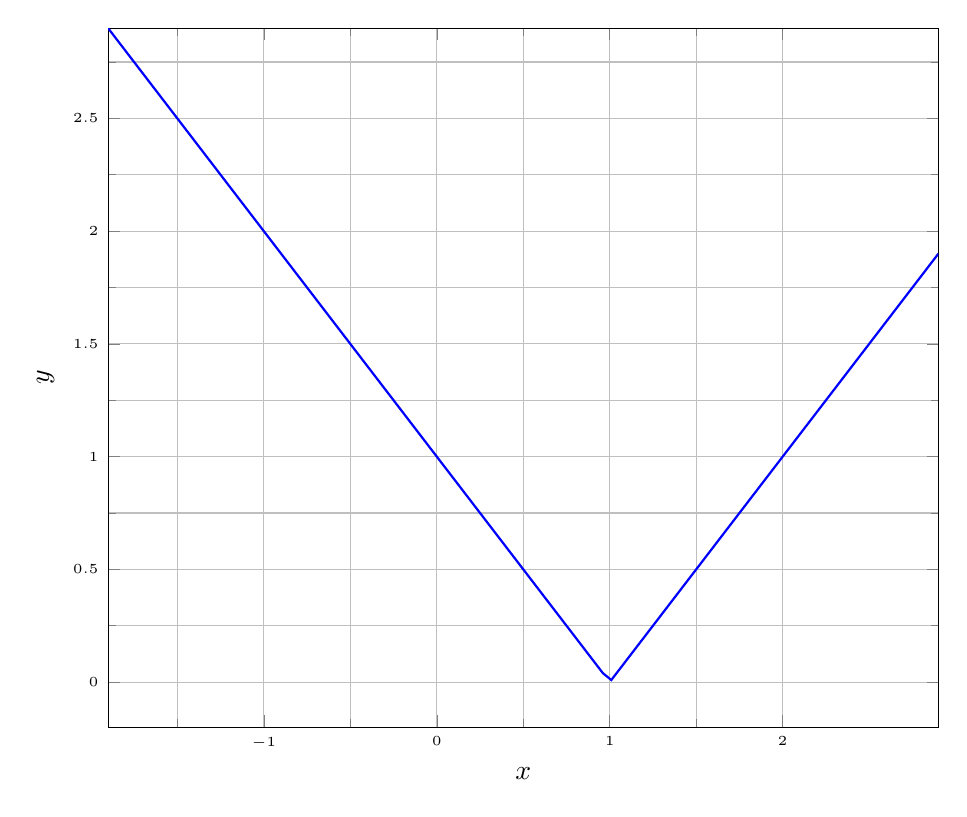
\begin{tikzpicture}
						\begin{axis}[minor tick num=1, ticklabel style={font=\tiny,fill=white}, xtick={-2,-1,0,1,2},
						xlabel={$x$},
						ylabel={$y$},xmax=2.9,xmin=-1.9,ymax=2.9,ymin=-0.2,width=1\textwidth,grid=both
						]
						\addplot[thick,blue,domain=-1.9:2.9,samples=100]{abs(x-1)};			
						\end{axis}
						\end{tikzpicture}
				\end{minipage}
			\end{enumerate}\vspace{-0.4cm}
		\subsection*{Definition: differenzierbar}
			\begin{tcolorbox}
				Wenn der \textbf{Differenzenquotient} an \underline{einer Stelle} $x_0$ existiert, so nennt man die Funktion\\
				
				\textbf{differenzierbar an der Stelle $x_0$}.
			\end{tcolorbox}
			\minisec{Aufgabe 2}
			 An welchen Stellen ist Funktion $f(x)=\left\vert x-1\right\vert$ differenzierbar. Begründen Sie Ihre Antwort anhand der Definitionen.\vspace{-0.3cm}
			\subsection*{Definition: Ableitungsfunktion}
			\begin{tcolorbox}
				Ist eine Funktion $f$ für alle $x\in D_f$ differenzierbar, so heißt die Funktion, die jeder Stelle $x$ der Definitionsmenge die Ableitung $f^\prime(x)$ an dieser Stelle zuordnet,\\
				
				\textbf{die Ableitungsfunktion} $f^\prime(x)$ oder kurz \textbf{Ableitung von} $f$.
				\tcblower
				  $f^\prime(x)$ wird \glqq f Strich von x\grqq gesprochen.  
			\end{tcolorbox}\vspace{-0.3cm}
			\minisec{Aufgabe 3}
			Petra behauptet die Funktion $f(x)=\left\vert x-1\right\vert$ besitzt trotzdem eine Ableitungsfunktion. Es muss lediglich eine Einschränkung vorgenommen werden.
			\begin{enumerate}[a)]
				\item Verwenden Sie die Lösung der Aufgabe 2 um eine Einschränkung vorzunehmen.
				\item Nennen Sie die Ableitungsfunktion. Sie können diese berechnen oder anhand der Abbildung begründen. \\

				\textit{Tipp: Die Ableitungsfunktion besteht aus zwei Funktionen mit unterschiedlichen Definitionsbereichen ($D_f$)}
			\end{enumerate}
			
\end{document}

